\documentclass{beamer}
%\usetheme{Madrid} % My favorite!
%\usetheme{Boadilla} % Pretty neat, soft color.
%\usetheme{default}
\usetheme{Warsaw}
%\usetheme{Bergen} % This template has nagivation on the left
%\usetheme{Frankfurt} % Similar to the default 
%with an extra region at the top.
\usecolortheme{seahorse} % Simple and clean template
%\usetheme{Darmstadt} % not so good
% Uncomment the following line if you want %
% page numbers and using Warsaw theme%
%\setbeamertemplate{footline}[page number]
\setbeamercovered{transparent}
%\setbeamercovered{invisible}
% To remove the navigation symbols from 
% the bottom of slides%
\setbeamertemplate{navigation symbols}{} 
\usepackage{epstopdf}
\usepackage{pgf}
\usepackage{tikz}
\usepackage{setspace} %Spacing
\usepackage{graphicx}
\usepackage{caption}
\usepackage{natbib}
\usepackage{wrapfig}
%\usepackage{subcaption}
\usepackage{enumerate}
\usetikzlibrary{positioning,shapes.geometric}
\usetikzlibrary{arrows}
\DeclareMathOperator*{\argmin}{arg\,min}

\usepackage{hyperref}
\hypersetup{
    colorlinks,
    citecolor=black,
    filecolor=black,
    linkcolor=blue,
    urlcolor=black
}


\newcommand{\Om}{\Omega}


\newcommand{\bs}[1]{\boldsymbol{#1}}
\newcommand{\wt}[1]{\widetilde{#1}}
\newcommand{\wh}[1]{\widehat{#1}}
\newcommand{\ol}[1]{\overline{#1}}
\newcommand{\e}{\varepsilon}
%\usepackage{bm}         % For typesetting bold math (not \mathbold)
%\logo{\includegraphics[height=0.6cm]{yourlogo.eps}}
%
\title[\texttt{Intro to Git}]{Introduction to Git}
\author[Asad Haris]{Asad Haris}
\institute[Dept of Biostatistics]
{Department of Biostatistics \\
University of Washington\\
\medskip
}
\date{\today}
% \today will show current date. 
% Alternatively, you can specify a date.
%
\begin{document}

\begin{frame}
\titlepage
\end{frame}

\begin{frame}
\frametitle{Step 0: Installation}
\begin{itemize}
\item \textbf{Install Git}: \url{https://git-scm.com/downloads}
\item \textbf{Easy Install for Linux}
\begin{itemize}
\item \texttt{apt-get install git} (Ubuntu/Debian)
\item \texttt{yum install git} (Fedora)
\item Others can be found at \url{https://git-scm.com/download/linux}
\end{itemize}

\item This is all we need to get started. You can work with Git completely off-line. 
%If you wish to follow this tutorial to the end, 

\pause
\item Make an account at 

\url{https://github.com/} or \url{https://bitbucket.org/} 

We will discuss differences between the two. 
\end{itemize}



\end{frame}


\begin{frame}
\centering
\Large While everything is downloading/installing... 
\end{frame}

\begin{frame}
\frametitle{What is Git?}
\begin{itemize}
\item Git is a version control system
\item As the name suggests, a system to manage different versions of a project
\item A project in Git is called a repository/repo 
\item Git allows us to take it a step further with many other features
\item Collaborating on a project is much simpler with Github/Bitbucket
\end{itemize}
\end{frame}

\begin{frame}
\centering
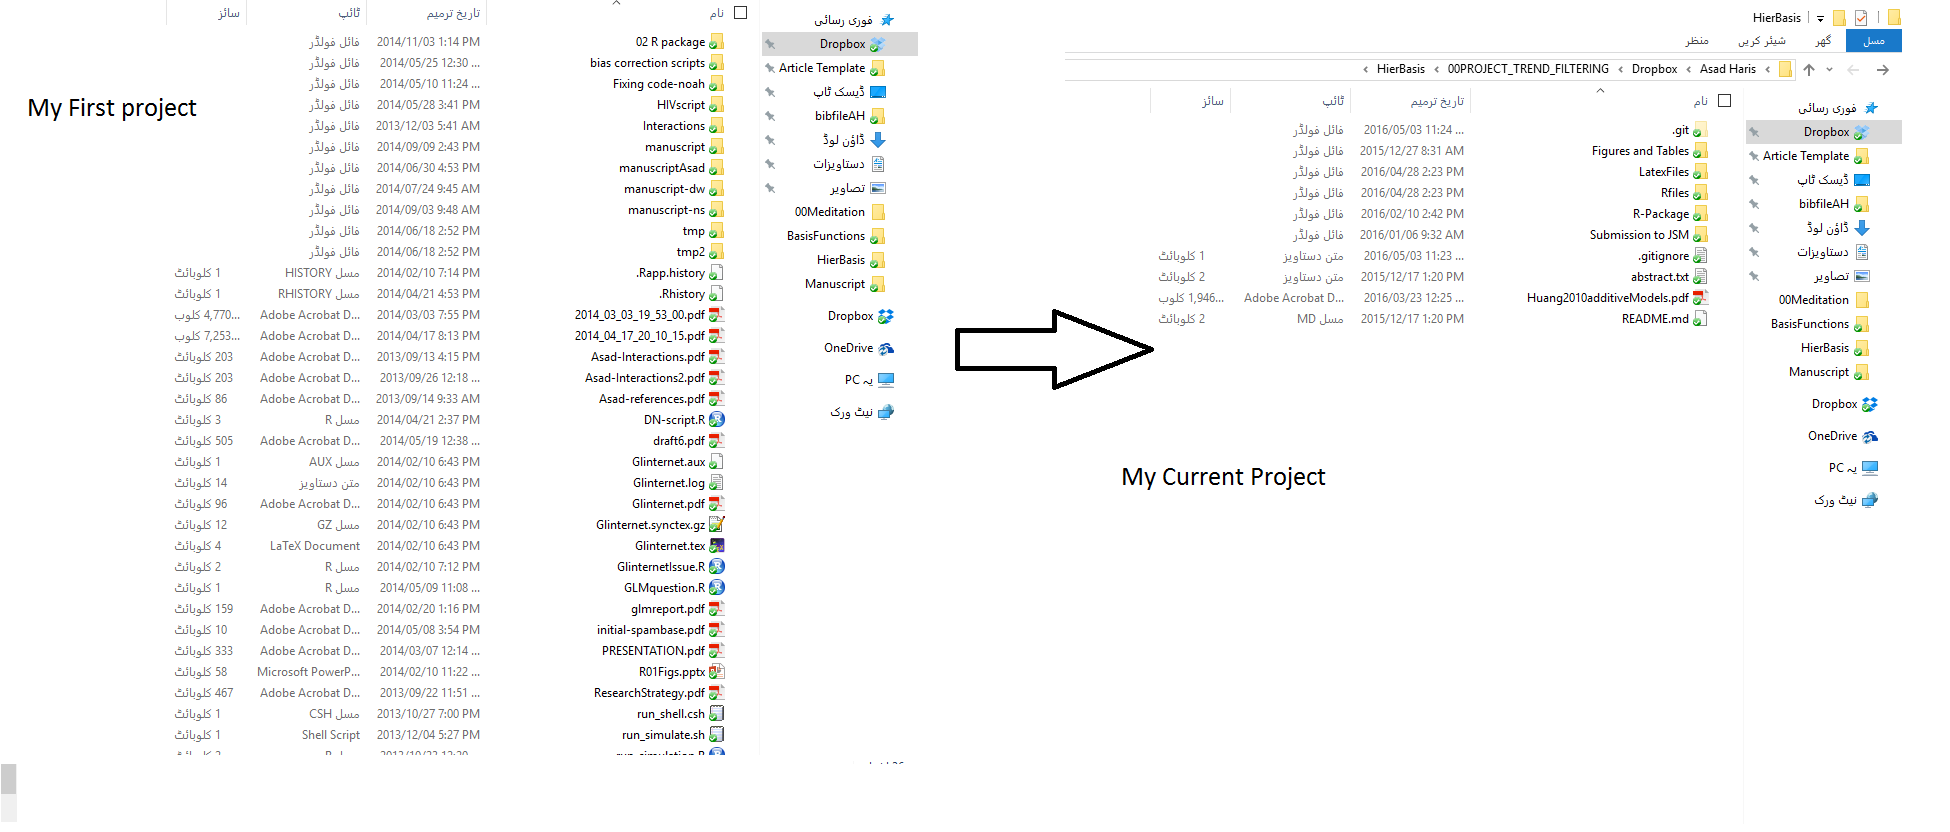
\includegraphics[scale = 0.25]{history}
\end{frame}


\begin{frame}
\frametitle{How does git work?}
\centering
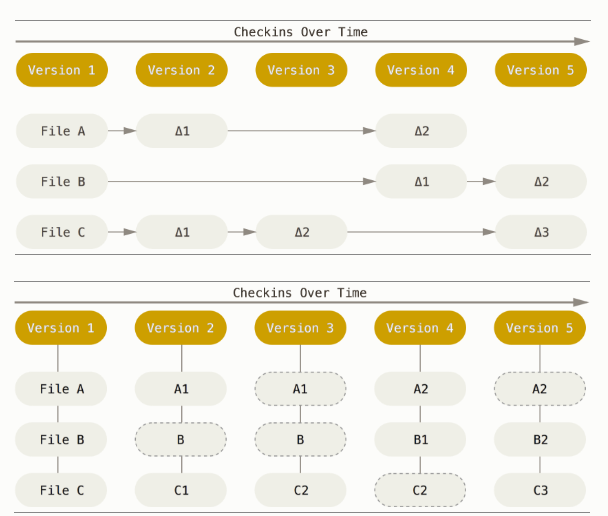
\includegraphics[scale = 0.5]{workflow}
\end{frame}

\begin{frame}
\frametitle{So why Git?}
\textbf{Advantages}
\begin{itemize}
\item Allows you manage different versions of your project
\item We can go back in time to previous versions 
\item Isn't restricted to specific type of projects (not just for computer scientists)
\item Makes collaboration on a project really easy
\item We have nice tools like GitHub and Bitbucket for collaboration and online sharing
\end{itemize}

\textbf{Disadvantages}
\begin{itemize}
\item Initial learning curve, which we will overcome today
\end{itemize}
\end{frame}


\begin{frame}
\frametitle{As promised Github vs. Bitbucket}
Essentially, Github/Bitbucket is a remote location to store/share your repositories


\begin{table}
\centering

\begin{tabular}{c|cc}
\hline
 & Github & Bitbucket\\
\hline
Cost & Free & Free\\
Public Repositories & Unlimited & Unlimited\\
Private Repositories & 5\footnote[1] & Unlimited\\
Collaborators & Unlimited & 5\footnote[2] \\
\end{tabular}
\caption{1. After student discount. 2. For the free account, can have upto unlimited collaborators with paid account.}
\end{table}

\end{frame}






\end{document} 